\begin{center}
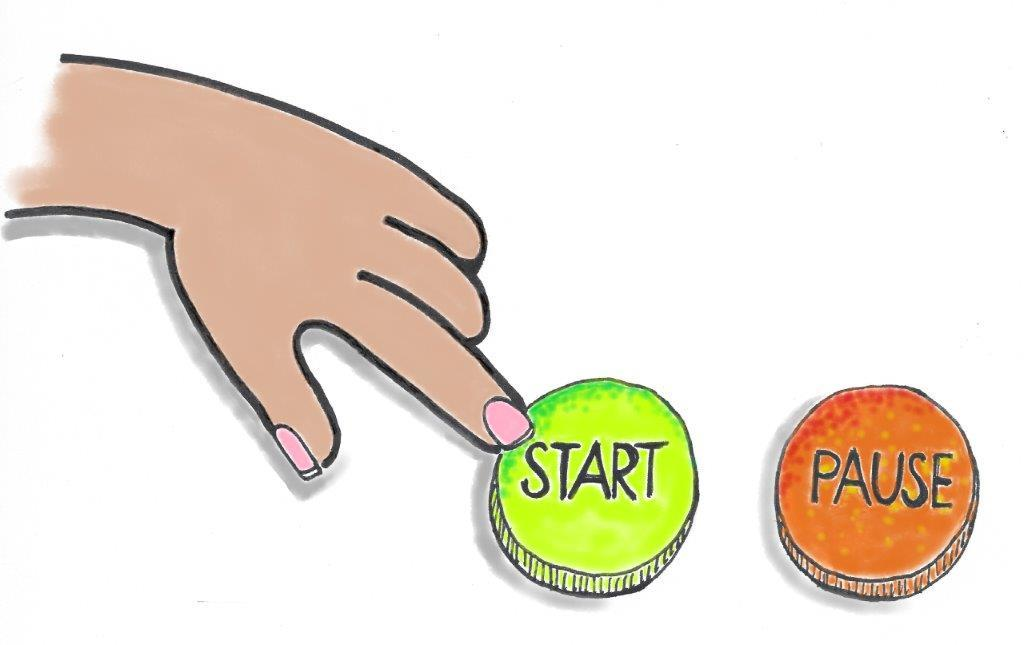
\includegraphics[width=0.8\textwidth]{content/3/chapter7/images/7.png}\\
Cippi starts the workflow
\end{center}

Before I create variations of the future from section co\_return, we should understand its control flow. Comments make the control flow transparent. Additionally, I provide a link to the presented programs on online compilers.

\hspace*{\fill} \\ %插入空行
\noindent
Control flow of an eager future
\begin{lstlisting}[style=styleCXX]
// eagerFutureWithComments.cpp

#include <coroutine>
#include <iostream>
#include <memory>

template<typename T>
struct MyFuture {
std::shared_ptr<T> value;
	MyFuture(std::shared_ptr<T> p): value(p) {
		std::cout << " MyFuture::MyFuture" << '\n';
	}
	~MyFuture() {
		std::cout << " MyFuture::~MyFuture" << '\n';
	}
	T get() {
		std::cout << " MyFuture::get" << '\n';
		return *value;
	}

	struct promise_type {
		std::shared_ptr<T> ptr = std::make_shared<T>();
		promise_type() {
			std::cout << " promise_type::promise_type" << '\n';
		}
		~promise_type() {
			std::cout << " promise_type::~promise_type" << '\n';
		}
		MyFuture<T> get_return_object() {
			std::cout << " promise_type::get_return_object" << '\n';
			return ptr;
		}
		void return_value(T v) {
		std::cout << " promise_type::return_value" << '\n';
		*ptr = v;
		}
		std::suspend_never initial_suspend() {
			std::cout << " promise_type::initial_suspend" << '\n';
			return {};
		}
		std::suspend_never final_suspend() noexcept {
			std::cout << " promise_type::final_suspend" << '\n';
			return {};
		}
		void unhandled_exception() {
			std::exit(1);
		}
	};
};

MyFuture<int> createFuture() {
	std::cout << "createFuture" << '\n';
	co_return 2021;
}

int main() {

	std::cout << '\n';
	
	auto fut = createFuture();
	auto res = fut.get();
	std::cout << "res: " << res << '\n';
	
	std::cout << '\n';

}
\end{lstlisting}

The call createFuture (line 60) causes the creating of the instance of MyFuture (line 59). Before MyFuture’s constructor call (line 10) is completed, the promise promise\_type is created, executed, and destroyed (lines 20 - 48). The promise uses in each step of its control flow the awaitable std::suspend\_never (lines 36 and 40) and, hence, never pauses. To save the result of the promise for the later fut.get() call (line 60), it has to be allocated. Furthermore, the used std::shared\_ptrs ensure (lines 9 and 21) that the program does not cause a memory leak. As a local, fut goes out of scope in line 65, and the C++ run time calls its destructor.

You can try out the program on the \href{https://godbolt.org/z/Y9naEx}{Compiler Explorer}.

\begin{center}
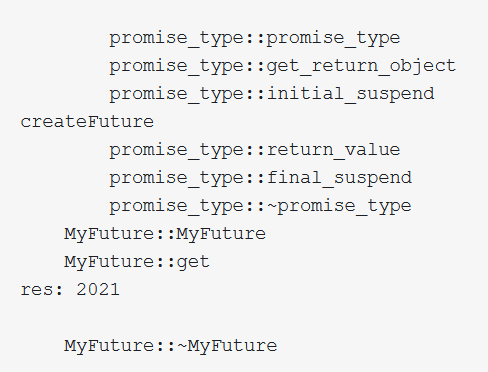
\includegraphics[width=0.8\textwidth]{content/3/chapter7/images/8.png}\\
An eager future
\end{center}

The presented coroutine runs immediately and is, therefore, eager. Furthermore, the coroutine runs in the thread of the caller.

Let’s make the coroutine lazy.

\subsubsubsection{7.2.1\hspace{0.2cm} A Lazy Future}

A lazy future is a future that runs only if asked for the value. Let’s see what I have to change in the eager coroutine, presented in eagerFutureWithComments.cpp, to make it lazy.

\hspace*{\fill} \\ %插入空行
\noindent
Control flow of a lazy future
\begin{lstlisting}[style=styleCXX]
// lazyFuture.cpp

#include <coroutine>
#include <iostream>
#include <memory>

template<typename T>
struct MyFuture {
	struct promise_type;
	using handle_type = std::coroutine_handle<promise_type>;
	
	handle_type coro;
	
	MyFuture(handle_type h): coro(h) {
		std::cout << " MyFuture::MyFuture" << '\n';
	}
	~MyFuture() {
		std::cout << " MyFuture::~MyFuture" << '\n';
		if ( coro ) coro.destroy();
	}
	
	T get() {
		std::cout << " MyFuture::get" << '\n';
		coro.resume();
		return coro.promise().result;
	}

	struct promise_type {
		T result;
		promise_type() {
			std::cout << " promise_type::promise_type" << '\n';
		}
		~promise_type() {
			std::cout << " promise_type::~promise_type" << '\n';
		}
		auto get_return_object() {
			std::cout << " promise_type::get_return_object" << '\n';
			return MyFuture{handle_type::from_promise(*this)};
		}
		void return_value(T v) {
			std::cout << " promise_type::return_value" << '\n';
			result = v;
		}
		std::suspend_always initial_suspend() {
			std::cout << " promise_type::initial_suspend" << '\n';
			return {};
		}
		std::suspend_always final_suspend() noexcept {
			std::cout << " promise_type::final_suspend" << '\n';
			return {};
		}
		void unhandled_exception() {
			std::exit(1);
		}
	};
};

MyFuture<int> createFuture() {
	std::cout << "createFuture" << '\n';
	co_return 2021;
}

int main() {

	std::cout << '\n';
	
	auto fut = createFuture();
	auto res = fut.get();
	std::cout << "res: " << res << '\n';
	
	std::cout << '\n';

}
\end{lstlisting}

Let’s first study the promise. The promise always suspends at the beginning (line 44) and the end (line 48). Furthermore, the member function get\_return\_object (line 36) creates the return object that is returned to the caller of the coroutine createFuture (line 58). The future MyFuture is more interesting. It has a handle coro (line 12) to the promise. MyFuture uses the handle to manage the promise. It resumes the promise (line 24), asks the promise for the result (line 25), and finally destroys it (line 19). The resumption of the coroutine is necessary because it never runs automatically (line 44). When the client invokes fut.get() (line 68) to ask for the result of the future, it implicitly resumes the promise (line 24).

You can try out the program on the \href{https://godbolt.org/z/EejWcj}{Compiler Explorer}.

\begin{center}
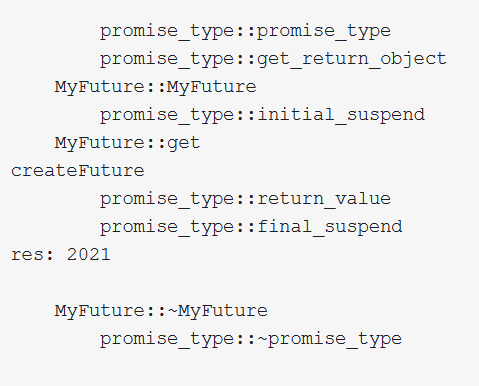
\includegraphics[width=0.8\textwidth]{content/3/chapter7/images/9.png}\\
A lazy future
\end{center}

What happens if the client is not interested in the result of the future? Let’s try it out.

\hspace*{\fill} \\ %插入空行
\noindent
The client does not resume the coroutine
\begin{lstlisting}[style=styleCXX]
int main() {
	
	std::cout << '\n';
	
	auto fut = createFuture();
	// auto res = fut.get();
	// std::cout << "res: " << res << '\n';
	
	std::cout << '\n';
}
\end{lstlisting}

As you may guess, the promise never runs, and the member functions return\_value and final\_suspend are not executed.

\begin{center}
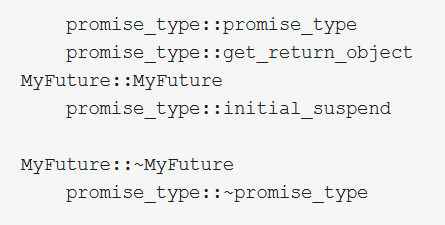
\includegraphics[width=0.8\textwidth]{content/3/chapter7/images/10.png}\\
A lazy future that is not started
\end{center}

\begin{tcolorbox}[breakable,enhanced jigsaw,colback=red!5!white,colframe=red!75!black,title={About the Numbers}]
One of the challenges of dealing with coroutines is to handle the lifetime of the coroutine. In the previous program eagerFutureWithComments.cpp, I stored the coroutine result in a std::shared\_ptr. This is critical because the coroutine is executed eagerly.

In this program lazyFuture.cpp, the call final\_suspend always suspends (line 48): std::suspend\_always final\_suspend(). Consequently, the promise outlives the client, and a std::shared\_ptr is not necessary anymore. Returning std::suspend\_never from the function final\_suspend would cause, in this case, undefined behavior because the client would outlive the promise. Hence, the lifetime of the result ends, bevor the client asks for it.
\end{tcolorbox}

Let’s vary the coroutine further and run the promise in a separate thread.

\subsubsubsection{7.2.2\hspace{0.2cm} Execution on Another Thread}

The coroutine is fully suspended before entering the coroutine createFuture (line 67), because the member function initial\_suspend returns std::suspend\_always (line 52). Consequently, the promise can run on another thread.

\hspace*{\fill} \\ %插入空行
\noindent
Executing the promise on another thread
\begin{lstlisting}[style=styleCXX]
// lazyFutureOnOtherThread.cpp

#include <coroutine>
#include <iostream>
#include <memory>
#include <thread>

template<typename T>
struct MyFuture {
	struct promise_type;
	using handle_type = std::coroutine_handle<promise_type>;
	handle_type coro;

	MyFuture(handle_type h): coro(h) {}
	~MyFuture() {
		if ( coro ) coro.destroy();
	}

	T get() {
		std::cout << " MyFuture::get: "
	              << "std::this_thread::get_id(): "
	              << std::this_thread::get_id() << '\n';
		std::thread t([this] { coro.resume(); });
		t.join();
		return coro.promise().result;
	}

	struct promise_type {
		promise_type(){
			std::cout << " promise_type::promise_type: "
			          << "std::this_thread::get_id(): "
			          << std::this_thread::get_id() << '\n';
		}
		~promise_type(){
			std::cout << " promise_type::~promise_type: "
			          << "std::this_thread::get_id(): "
			          << std::this_thread::get_id() << '\n';
		}
		
		T result;
		auto get_return_object() {
			return MyFuture{handle_type::from_promise(*this)};
		}
		void return_value(T v) {
			std::cout << " promise_type::return_value: "
			          << "std::this_thread::get_id(): "
			          << std::this_thread::get_id() << '\n';
			std::cout << v << std::endl;
			result = v;
		}
		std::suspend_always initial_suspend() {
			return {};
		}
		std::suspend_always final_suspend() noexcept {
			std::cout << " promise_type::final_suspend: "
			          << "std::this_thread::get_id(): "
			          << std::this_thread::get_id() << '\n';
		return {};
		}
		void unhandled_exception() {
			std::exit(1);
		}
	};
};

MyFuture<int> createFuture() {
	co_return 2021;
}

int main() {

	std::cout << '\n';
	
	std::cout << "main: "
	<< "std::this_thread::get_id(): "
	<< std::this_thread::get_id() << '\n';
	
	auto fut = createFuture();
	auto res = fut.get();
	std::cout << "res: " << res << '\n';
	
	std::cout << '\n';

}
\end{lstlisting}

I added a few comments to the program that show the id of the running thread. The program lazyFutureOnOtherThread.cpp is quite similar to the previous program lazyFuture.cpp. The main difference is the member function get (line 19). The call std::thread t([this] \{ coro.resume(); \}); (line 24) resumes the coroutine on another thread.

You can try out the program on the \href{https://wandbox.org/permlink/jFVVj80Gxu6bnNkc}{Wandbox} online compiler.

\begin{center}
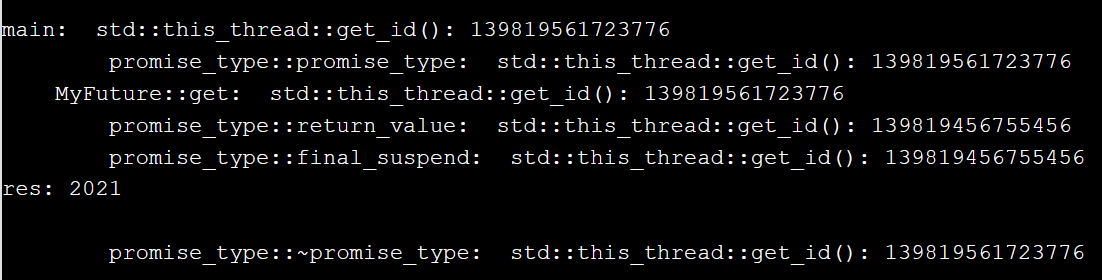
\includegraphics[width=0.8\textwidth]{content/3/chapter7/images/11.png}\\
Execution on another thread
\end{center}

I want to add a few additional remarks about the member function get. It is crucial that the promise, resumed in a separate thread, finishes before it returns coro.promise().result.

\hspace*{\fill} \\ %插入空行
\noindent
The member function get using std::thread
\begin{lstlisting}[style=styleCXX]
T get() {
	std::thread t([this] { coro.resume(); });
	t.join();
	return coro.promise().result;
}
\end{lstlisting}

Where I to join the thread t after the call return coro.promise().result, the program would have undefined behavior. In the following implementation of the function get, I use a std::jthread. Since std::jthread automatically joins when it goes out of scope. This is too late.

\hspace*{\fill} \\ %插入空行
\noindent
The member function get using std::jthread
\begin{lstlisting}[style=styleCXX]
T get() {
	std::jthread t([this] { coro.resume(); });
	return coro.promise().result;
}
\end{lstlisting}

In this case, the client likely gets its result before the promise prepares it using the member function return\_value. Now, result has an arbitrary value, and therefore so does res.

\begin{center}
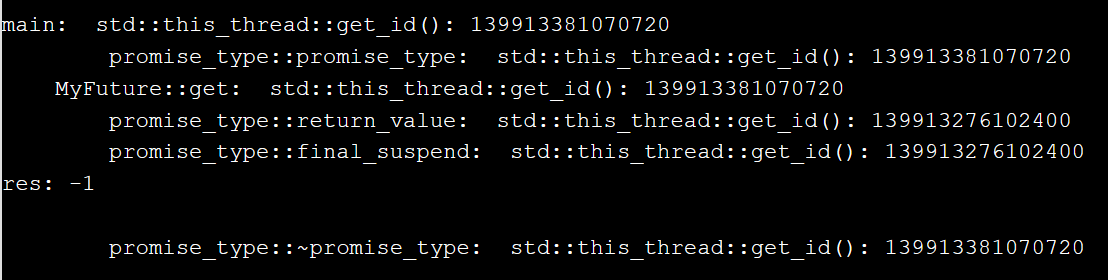
\includegraphics[width=0.8\textwidth]{content/3/chapter7/images/12.png}\\
Execution on another thread
\end{center}

There are other possibilities to ensure that the thread is done before the return call.

\begin{itemize}
\item 
Create a std::jthread in its scope.

\hspace*{\fill} \\ %插入空行
\noindent
std::jthread has its own scope
\begin{lstlisting}[style=styleCXX]
T get() {
	{
		std::jthread t([this] { coro.resume(); });
	}
	return coro.promise().result;
}
\end{lstlisting}

\item 
Make std::jthread a temporary object

\hspace*{\fill} \\ %插入空行
\noindent
std::jthread as a temporary
\begin{lstlisting}[style=styleCXX]
T get() {
	std::jthread([this] { coro.resume(); });
	return coro.promise().result;
}
\end{lstlisting}

\end{itemize}

In particular, I don’t like the last solution because it may take you a few seconds to recognize that I just called the constructor of std::jthread.
